%
% $Id: chapter2.tex 2612 2008-06-03 18:32:54Z jozinke $
%

\chapter{Background} \label{sec:background}

The following section introduces the concept of \ac{HIDS} with the specific example of Fail2ban and presents the problem setting 
this thesis aims to solve. In addition to that, a short overview over common types of inter process communication and existing \ac{IPC} based logging solution is given. 
Finally, external libraries and other software used for the implementation and evaluation of the proof of concept \ac{IPS} are introduced.    

\section{Host-based Intrusion Detection / Prevention} \label{sec:hids}

Intrusion Detection Systems are tasked with monitoring and collecting data from target systems, which is then further processed and analyzed, to identify 
potential threads and facilitate a response \cite{vigna2006}.
The idea of specialized software for detecting intrusion attempts and other 
security threads goes as far back as 1980, when James Anderson published a study on 
``Computer security threat monitoring and surveillance''\cite{anderson1980}. It defined a thread to a computer systems as the: ``potential possibility of a deliberate unauthorized attempt to access or manipulate information
op render a system unreliable or unusable''\cite[p.6]{anderson1980}. Further, he suggested the use of automated tools to assist with security monitoring. In 1987, Dorothy
Denning presented a seminal model for Intrusion Detection Systems, that proposed the use of pattern matching based on
statistical analysis of audit records generated by a system, in order to detect abnormal user behavior \cite{denning1987}. 
Intrusion Detection Systems in general, can collect data from a multitude of sources. This allows for the distinction between \acp{NIDS} and Host-based Introduction Detection Systems. \ac{NIDS}
monitor network interfaces and analyze captured traffic, while \ac{HIDS} gather information directly provided by the hosts under their supervision. For the latter, this includes event logs of applications, as well as \ac{OS} based information,
such as user logins, file system operations or systemcalls. For analysis of the accumulated data, there a two commonly deployed strategies: 1. Misuse based detection relies on predefined 
patterns of misuse or malicious behavior, which are then matched against the observed data. 2. Anomaly based detection uses statistical analysis, to identify significant deviations
from normally observed behavior, which, in principal, enables the detection of attack patterns, that have not been previously observed. \cite{vigna2006} 

\subsection{Fail2ban} \label{sec:fail2ban}

Fail2ban is a open source Intrusion Prevention System \ac{IPS}, that is widely used to protect hosts against a range of network-based attacks, such as for instance, brute-force login attempts\cite{fail2ban}. Intrusion prevention system constitute
a special class of \ac{IDS}, that not only detects an intrusion attempt, but also initiates an active response, with the aim of preventing or mitigating the attack. To identify potentially malicious clients,
Fail2ban uses a misuse detection approach based on application logs. For configured applications, Fail2ban actively monitors their log and parses new entries based on a predefined filter. Fail2ban uses configuration units called `jails'  
, that allow for the customization to different applications. A jail defines a path to an application log, the filter being applied to the log messages within the logfile and an action, that
is executed on client matching the filter criteria. In addition to that, jails contain further parameters, such as the threshold of matches per client for the action to be executed,
as well as the duration of the action. The filter component of a jail defines a set of regular expressions, that are used to identify certain events in a log, for example an unsuccessful login attempts or the 
exceeding of a request rate limit. The filter also obtains a clients IP address to identify the client and datetime information to determine, if the event occurred within a relevant time frame. 
Most commonly, the action issued by Fail2ban for eligible clients, is to ban the clients IP address. Fail2ban facilitates this via an \texttt{iptables} entry. 
texttt{Iptables} is a utility program for Linux systems, that allows the interaction with the \texttt{netfilter} kernel framework to implement packet filtering rules \cite{netfiler,iptables}. When banning a client, Fail2ban add a iptables rule for the clients IP address that leads 
to the dropping of all subsequent network packets from that address, for as long as the rule is active.
\par
Fail2bans netfilter-based approach of packet filtering has the disadvantage of scaling poorly for large traffic rates, since packets need to traverse several processing steps of the kernel network stack before they are ultimately discarded.
In his master thesis, Florian Mikolajczak proposed the alternative usage of eBPF programs, as a more efficient way of implementing packet filtering for intrusion prevention systems\cite{mikolajczak2022}. The extended Berkley Packet Filter \ac{eBPF}      
is an interface of the Linux kernel, that allows the event based execution of verified, user defined programs within the kernel. Packet filtering through \ac{eBPF} can be facilitated with an \ac{eBPF} program,
that is executed on incoming packets and delivers a verdict, of wether the packets should be dropped or further processed by the Kernel. Via the \ac{XDP}, \ac{eBPF} programs can be attached to different hooks in 
the packet processing pipeline. For supported devices, programs can be attached in \texttt{XDP\_DRIVER} mode, where they are executed as part of the network device diver routine, very early into the packet processing. Florian Mikolajczak adapted an existing \ac{eBPF} program by Jesper Brouer
and Andy Gospodarek to handle \ac{IPv6} traffic as well and integrated it with Fail2ban to replace netfilter-based packet filtering. While he was able to demonstrate significant performance improvements over netfilter-based filtering, his measurements 
revealed, that Fail2ban has significant performance issues, when faced with a large influx of log messages. 

\begin{figure}[h!]
	\label{fig:fail2ban:mikolajczak2022}
	\centering
	\scriptsize
    \centerline{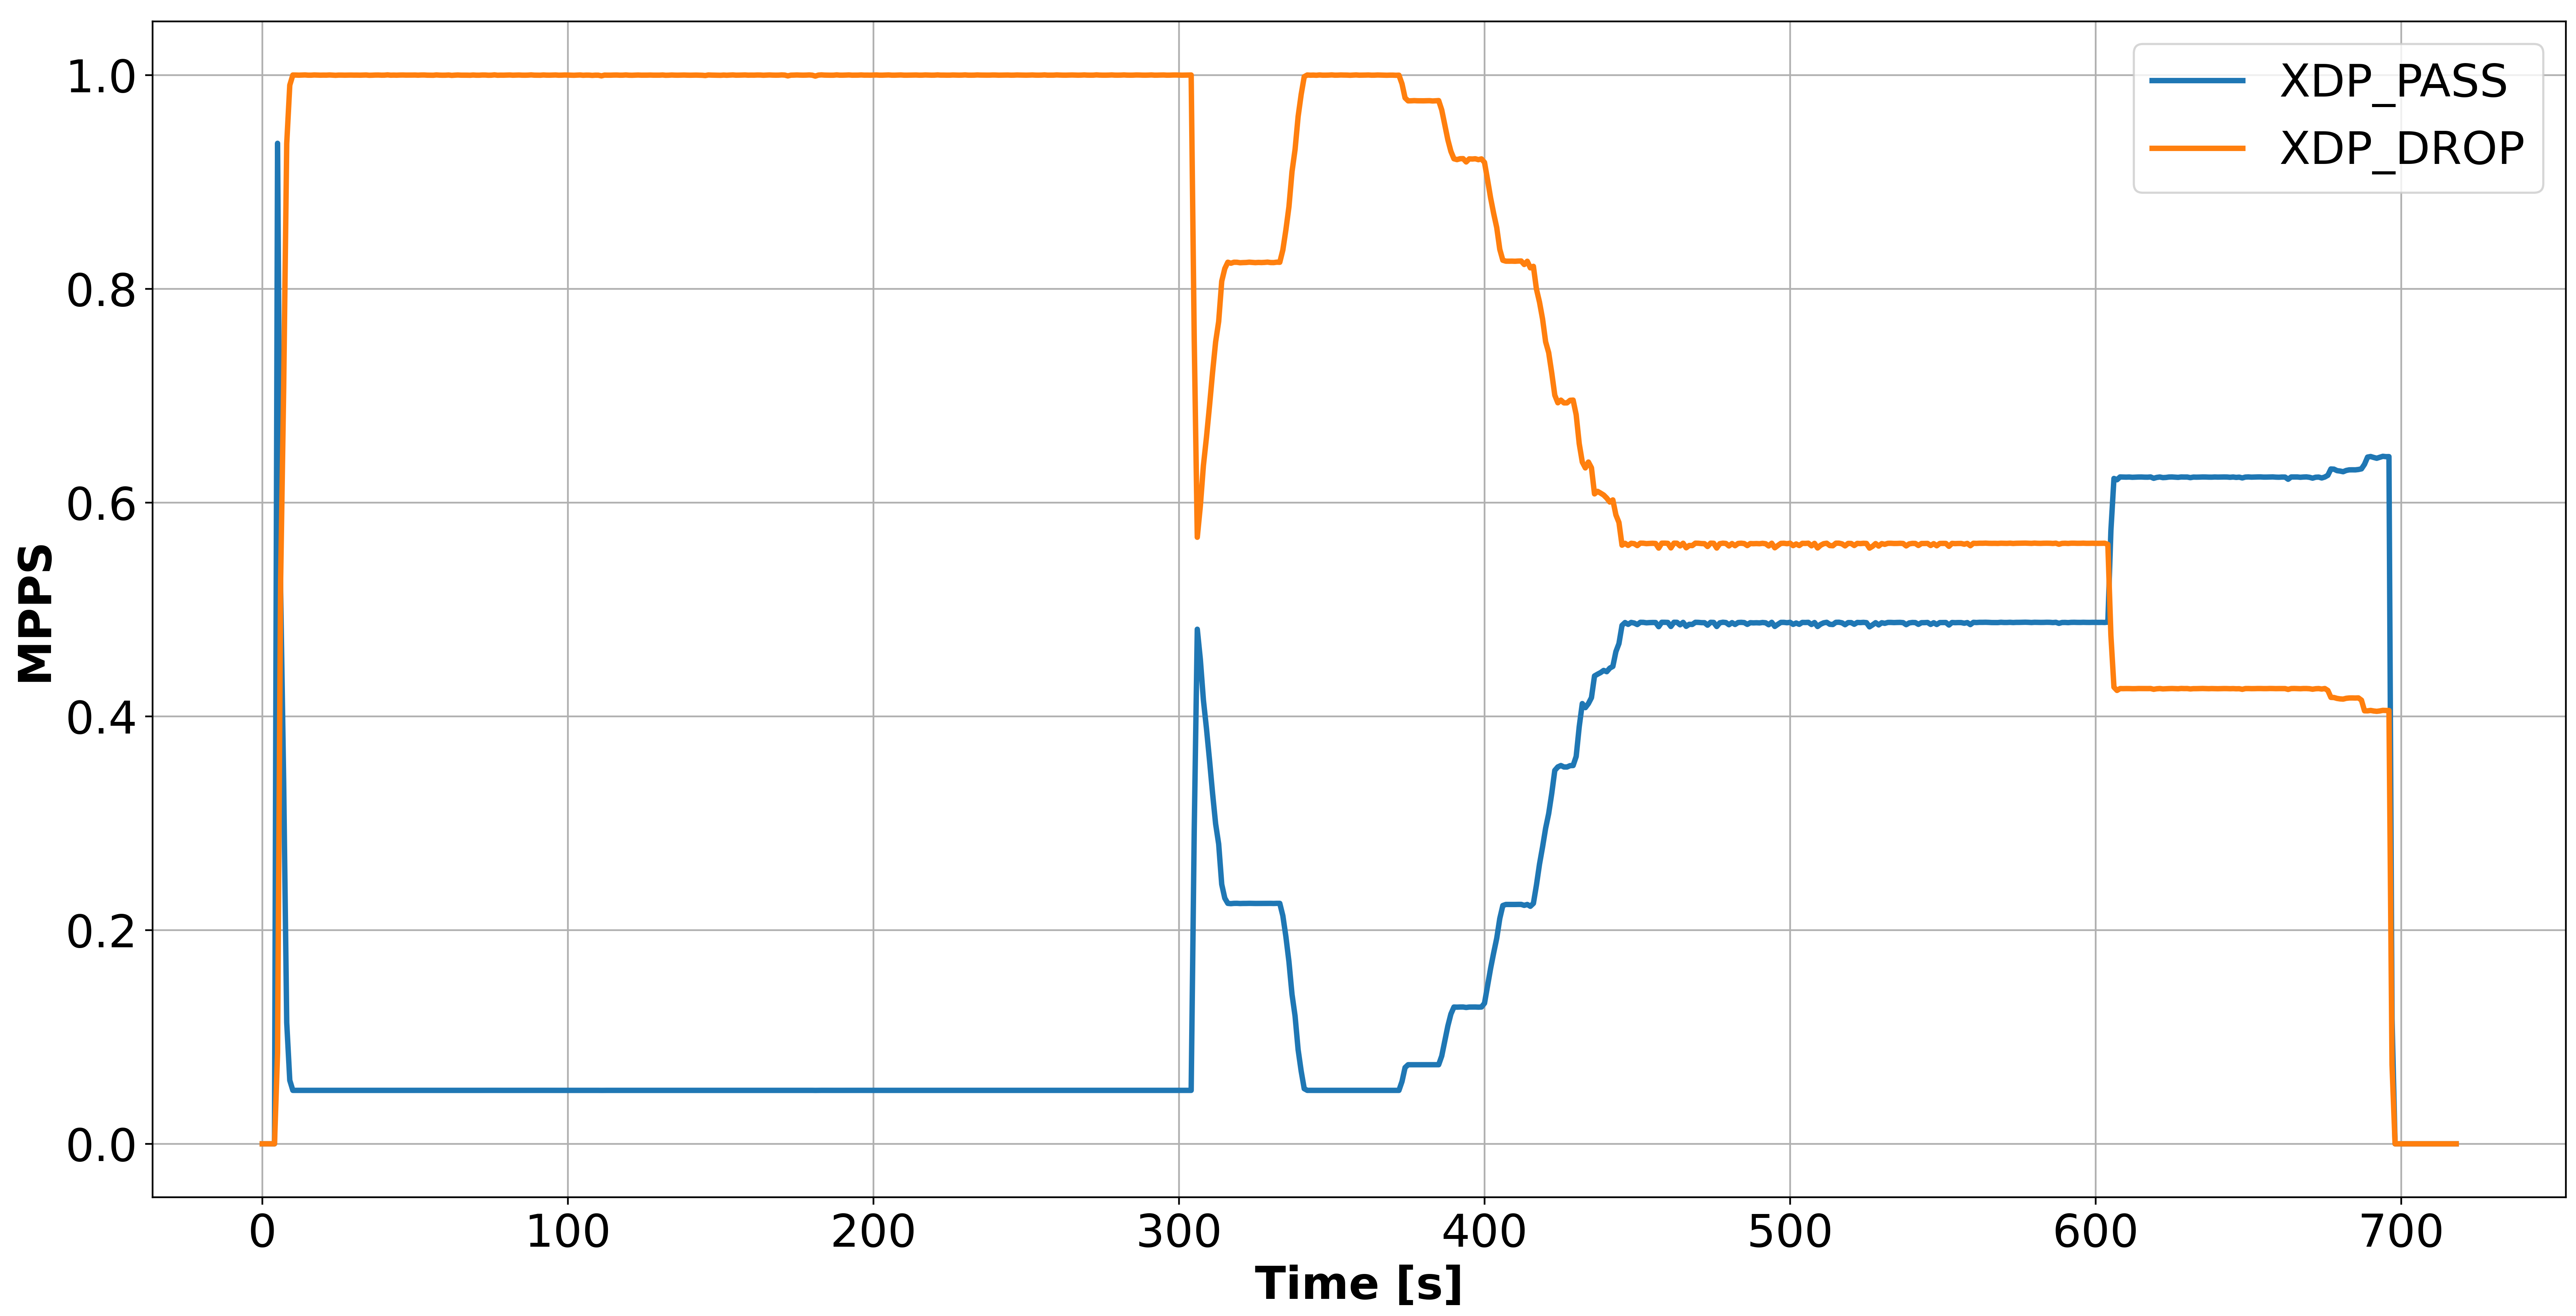
\includegraphics[width=1.2\textwidth]{images/Fail2Ban2.png}}
    \caption[Fail2ban measurement by \cite{mikolajczak2022}]{Results of experiment 1 from the  master thesis of Florian Mikolajczak\cite{mikolajczak2022}. Fail2Ban, even in conjunction with more efficient \ac{eBPF} filtering, performs poorly for large traffic rates.}
\end{figure}

Figure \ref{fig:fail2ban:mikolajczak2022} shows the results of the Fail2ban measurement conducted by Florian Mikolajczak. In the experiment, a BIND DNS Server received unwanted requests at a rate of 1 million \ac{PPS} from 254 different clients,
which resulted in corresponding entries in the servers rate-limit log. Fail2ban was configured to ban clients with rate limit violations for 300 seconds. Initially, the performance was as expected. However, after 
the end of the first ban cycle, Fail2ban failed to renew the ban for some clients, leading to a significant amount of unwanted traffic still reaching the application. Closer inspection of Fail2bans behavior indicated,
that the performance issues are likely the result of slow logfile parsing. Fail2bans rate of processing log entries appeared to be exceeded by rate of new entries, leading to Fail2ban falling increasingly further behind
in the processing of logged events. This constitutes a problem, as it essentially makes Fail2ban and by extension the protected host, vulnerable to \ac{DOS} attacks. This problem setting provides the primary motivation for this
thesis and is aimed to be resolved with the new \ac{IPC} architecture that will be developed.

\section{Inter-Process Communication}
\label{sec:ipc}

\subsection{Types of IPC}
\label{sec:ipc_types}

Inter-process communication allows the exchange of data between different processes through \acp{API} provided by the operating system. Since the
the development environment for this thesis will be Linux, the focus is restricted to \ac{IPC} APIs that are available on UNIX-like systems.
\minisec{Shared Memory}
A commonly used mechanism for sharing large amount of data between two processes on the same system is shared memory \cite[p.301ff.]{stevens1998ipc}.
Shared memory allows the allocation of a memory segment in RAM, that can mapped into address space of several processes. The memory segment has associated file associated permissions, 
allowing the creating process to control the read and write access of other processes. Linux provides two main ways of creating
shared memory in the System V shared memory \ac{API} \cite{systemvshm} and the newer POSIX shared memory \ac{API} \cite{posixshm}. Processes can essentially treat shared memory like 
any other valid memory in their address space, which allows for fast and flexible application. A disadvantage of shared memory, at least for the aforementioned APIs, is its restriction 
to the local system boundaries, though solutions for network based remote direct memory access (RDMA) exist\cite{recio2007}.
\par 
\minisec{Named Pipes / FIFOs}
Pipes, specifically named pipes, are a way of facilitating unidirectional data transfer between processes on a UNIX system. Named pipes have specific read and write file descriptors and are  
associated with a special file in the filesystem, which can be accessed by different processes. Pipe can be written to and read from via the write and read system calls. The data is transmitted in 
a \ac{FIFO} manner, hence why named pipes are also commonly referred to as FIFOs. The maximum capacity up to which a pipe can buffer data is limited, which by default is 65535 bytes on linux, but can be adapted by a user. \cite{pipe}   
\par
\minisec{Sockets}
Sockets are another common\ac{ICP} type for data transfer, that allow for one-to-one as well as one-to-many 
communication via a range of protocols\cite[p.57ff.]{stevens1998sock}. Sockets send data in formatted packets, that can be transmitted on a local host or via a network. For communication on a local system, UNIX systems offer UNIX Domain sockets. UNIX Domain sockets can be bound to a valid path in the filesystem, which serves as a way of addressing
the socket from another processes \cite{unixsock}. For data transfer beyond the local system, the Internet protocol \ac{IP} in conjunction with the Transmission Control Protocol \ac{TCP} or User Datagram 
Protocol \ac{UDP} is most common. TCP offers connection oriented data transmission, that requires an orderly connection establishment through a handshake between the commutating parties. It further ensures a reliable transfer of data, by       
detecting transmission errors trough acknowledgment and retransmitting unacknowledged packets. \ac{UDP} in contrast, provides no guarantees on reliable transfer, with the benefit of lower latency and less communication overhead. \cite[p.29ff.]{stevens1998sock}
\par
\minisec{Message Queues}
Finally, message queues are another commonly used \ac{IPC} mechanism that allow the exchange of messages between processes. Linux natively supports the System V \cite{systemvshm} and POSIX \cite{posixmsq} message queue APIs, but third party
implementations exist as well, for instance the ZeroMQ library \cite{zeromq}. Message queues essentially function as a buffer, which can store messages up to a certain capacity. A writing process adds messages to the queue, while
reading processes remove messages from the queue. Unlike with sockets, writing and reading can occur asynchronously i.e. messages do not have to be read immediately after being added to a queue. ZeroMQ specifically supports a range of communication 
patterns, among them the publish-subscribe pattern, where a writer sends messages to multiple subscribed readers or the request-reply pattern, that can be used to implement remote procedure calls.         

\subsection{IPC based logging} \label{sec:ipc_logging}
Other than traditional file-based logging, syslog is a commonly used protocol to facilitate network based-logging
on UNIX-based systems. The syslog protocol was first developed in the 1980s by Eric Allman, as a solution
for centralized logging and ultimately standardized by RFC 5424\cite{gerhards2009}. Syslog operates on a server-client
basis, where logging clients send messages to a syslog server, that can be located on the host or a remote machine. This allows 
the aggregation of log events from different sources and also serves to functionally separate the generation of log messages from storing, analyzing
and further processing. 
Syslog messages have a standardized format, that contains sender information, date and time of the event, as well as a facility and severity code. The facility indicates
the category of the logging application, while the severity indicates urgency and impact of the logged event\footnote{A full list of codes can be found in \cite[p.10-11]{gerhards2009}}. 
The syslog protocol is most commonly used with \ac{UDP} but does not specify a transport protocol and can also be used in 
encrypted form, via the \ac{TLS} protocol. 
Rsyslog is a modern implementation and extension of the syslog protocol developed by Rainer Gebhards\cite{rsyslog}.
It is intended as a high-performance log processing system for enterprise systems, that allows the aggregation of log events
from a variety of sources such ase files, named pipes, sockets or message queues via the \ac{AMQP}\cite{vinoski2006advanced}. 
\par
Logstash is another commonly used system, that supports \ac{IPC} based data aggregation \cite{logstash}. It provides input 
plugins for a range of inputs including files, sockets, pipes and messages queues. Logstash is part of the Elasticsearch technology stack, that allows 
distributed aggregation, processing and analysis of various data sources. Log aggregators like Rsyslog and Logstash have application in a security context,
as they can be integrated as part of \ac{SIEM} systems. \ac{SIEM} systems collect data from various security relevant contexts, such as firewalls or intrusion detection 
systems, to provide comprehensive real-time security monitoring and analysis of complex systems\cite{bhatt2014operational}.
\par
Regarding other high performance logging systems, the literature is, to the best of my knowledge, rather slim.
Jeong et al. present a shared memory based logging system for embedded UNIX-based applications \cite{jeong2013high}.
They use a memory mapped file to buffer log messages between the logging application and a daemon processes for forwarding the messages.
Their logging systems achieves a 10 times larger message throughput and 100 times lower latency than traditional syslog, which they attribute 
to the pure use of user-level \ac{IPC} that avoids costly context switches to the kernel. 


\section{External Software} \label{sec:software}

\subsection{Hyperscan} \label{sec:hyperscan}
 
Hyperscan is a open source regular expressions matching engine developed by Intel \cite{hyperscan}. 
It is specifically designed for high performance use cases, such as the application in security contexts and is being used by the intrusion detection systems Snort and Suricata.  
The process of regular expressions matching with Hyperscan is separated into compile- and run-time. At compile-time, a set regular expressions in string representation are compiled into a 
database, with additional configuration options. These include the processing mode, which 
can be streaming, block or vectored mode. Streaming mode allows the scanning of a continuous data stream,
which is facilitated via a state maintained between function calls. Block and vectored mode operate on data
that is readily available and can be scanned in a single call. Other compile options include 
case less and multiline scanning as well as instruction Hyperscan to only match an expression
once or to report the leftmost start index of a match\footnote{By default, only the end index of a match is provided.}. The latter comes with detrimental performance implications
Hyperscan allows the compilation
of multiple patterns into a database, which can be scanned for in parallel. 
For scanning hyperscan allows the user to define a callback function that is 
called when a match occurs. The matched pattern can be identified with an id parameter.
\par 
For the purpose of this thesis, Hyperscan will be used as a regular expression engine for
the matching of patterns in log messages received by the proof of concept \ac{IPS}.    

\subsection{io\_uring} \label{sec:io_uring}

io\_uring is an asynchronous \ac{IO} framework of the Linux kernel, that was first introduced in kernel version 5.1 \cite{io_uring}.
In contrast to traditional read and write systemcalls, io\_uring provides a non-block writing to or reading to
file descriptors. This is facilitated via an in memory queues, that are shared between a user process and the kernel.
The first queue is a submission queue, that the application uses to register \ac{IO} operations to the
kernel. The second queue is a completion queue, that the kernel fills with information on completed \ac{IO} requests.
An application can register several \ac{IO} operations, which are ultimately submitted to the kernel. The application
The application can then continuous execution, while the \ac{IO} operation is asynchronously executed by the kernel.
Via the completion queue, the application can poll the status of the submitted operations
and receive information about their completion.        
\par
Liburing is a library written by Jens Axboe, that provides a high level interface to the io\_uring framework \cite{liburing}.
It allows the setup of a a io\_uring instance, which can be subsequently used to conduct \ac{IO} operations
on files but also other types of file descriptors such as sockets.
\par
For the purpose of this thesis, liburing will be used to implement asynchronous file reading and writing
for both the proof concept \ac{IPS} as well as auxiliary applications. 

\subsection{Trex} \label{sec:trex}

TRex is a traffic generating tool developed by Cisco System \cite{trex}. It supports the generation of both
stateless as well stateful traffic, from network up to application layer protocols. TRex is build with the Data Plane Development Kit framework,
that offers user space based packet acceleration, enabling TRex to reach traffic rates up to 200Gbs, given appropriate hardware support. 
Traffic can be generated either via pcap files or Python scripts, using the packet manipulation library scapy \cite{scapy}.
\par 
For the purpose of this thesis, TRex will be used to conducted measurements and evaluate the proof of concept \ac{IPS}.
During initial measurements, its was discovered, that TRex struggles to maintain the advertised traffic rates for stateful traffic in certain scenarios.
More specifically, the absence of an acknowledgment packet to a \ac{TCP}-syn packet sent by TRex appears to inhibit performance.
Hence, measuring a \ac{DoS} scenario as described in section \ref{sec:fail2ban} for \ac{TCP} based traffic is problematic, as syn packet for banned clients
emulated by TRex will not be answerer by server protected by Fail2ban or the proof of concept \ac{IPS}. For this reason, all measurements conducted in this
thesis will be \ac{UDP} based.

